%%% A %%%
\subsection{External Interface Requirements}

	\subsubsection{User Interfaces}				
		The interface of our System is thought to be used via mobile app, because all the functionality make sense only in a \textit{movable} context (meaning, such that the user can do them anywhere they have an internet connection).

We will now list some of the user interfaces thought for \textit{Travlendar+}":

% login %
\begin{figure}[h]
	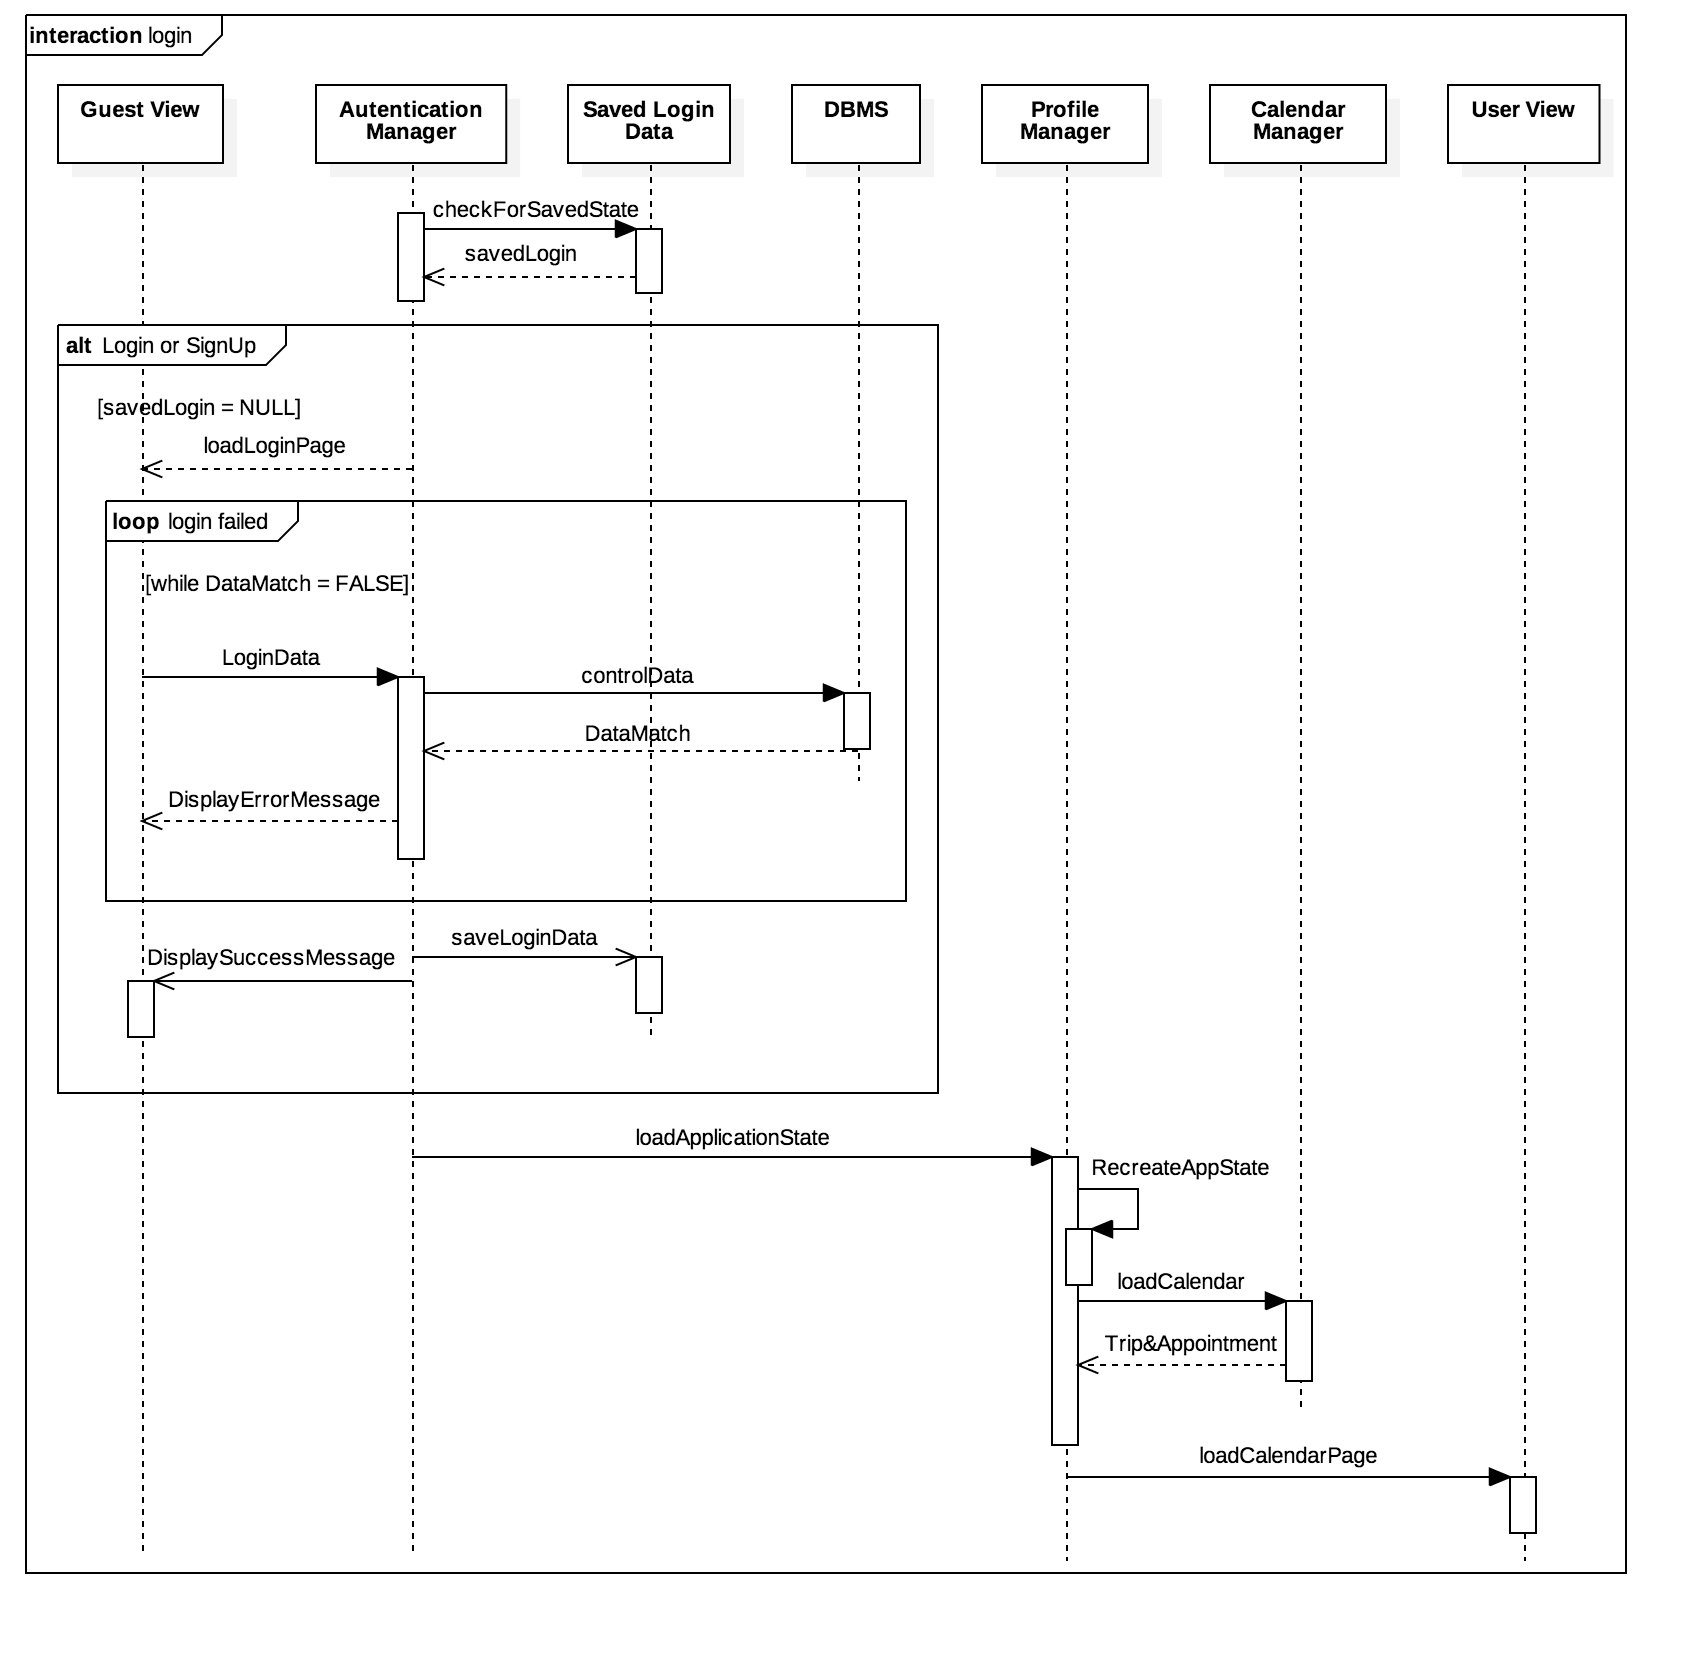
\includegraphics[width=5cm, height=9.5cm]{mockup/login}
	\centering
	\caption{Login Page.}
	\label{fig:login}
\end{figure}
As mentioned before, a \textit{Guest} or a \textit{non logged User} will encounter page showed in figure \ref{fig:login}, and he will never enter into the app until he completes the Registration or the Login procedures (see sections \ref{register_useCase} and \ref{login_useCase}).
% home page %

\begin{figure}[H]
	\begin{subfigure}{0.5\textwidth}
		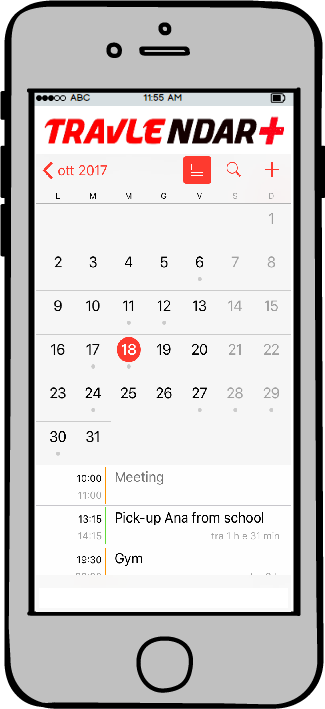
\includegraphics[width=5cm, height=9.5cm]{mockup/homepageMonth} 
		\centering
		\caption{Home Page in Monthly view.}
		\label{fig:homePage_Month}
	\end{subfigure}
	\begin{subfigure}{0.5\textwidth}
		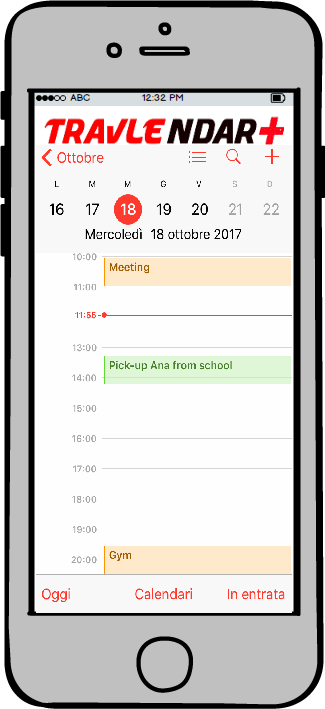
\includegraphics[width=5cm, height=9.5cm]{mockup/homepageDaily} 
		\centering
		\caption{Home Page in Daily view.}
		\label{fig:homePage_Day}
	\end{subfigure}
\end{figure}

% create Event %
\begin{figure}[h]
	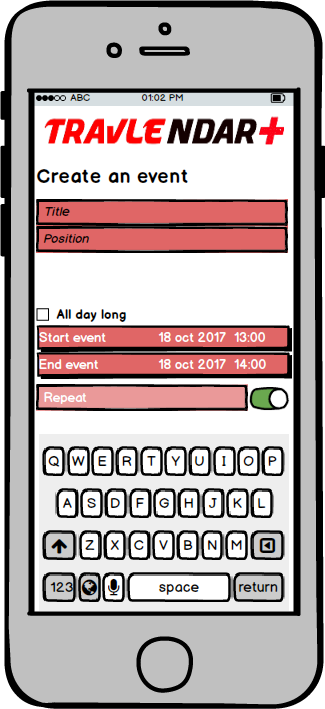
\includegraphics[width=5cm, height=9cm]{mockup/createAnEvent}
	\centering
	\caption{Create an Appointment page.}
	\label{fig:createEvent}
\end{figure}

\vfill
	
	\subsubsection{Hardware Interfaces}
		The system allows to interact with all the possible processors that are in the devices of the two companies Android and Apple. Among the most important processors there are: Qualcomm, ARM and Exynos.

	\subsubsection{Software Interfaces}
		\hfill		
		\begin{enumerate}
			\item Android
				\begin{itemize}
					\item[-] Name: Lollipop
					\item[-] Version: 5.0+
					\item[-] Source: \url{https://www.android.com/intl/it_it/versions/lollipop-5-0/}
				\end{itemize}
								
			\item Apple
				\begin{itemize}
					\item[-] Name: iOS
					\item[-] Version: 8.0+
					\item[-] Source: \url{https://www.apple.com}
				\end{itemize}
								
			\item Google Maps APIs
				\begin{itemize}
					\item[-] Name: Google Maps APIs
					\item[-] Source: \url{https://developers.google.com/maps/}
				\end{itemize}
		\end{enumerate}
			
	\subsubsection{Communication Interfaces}
		The system also interface with the applications for the use of sharing and payment services
		\hfill
		\begin{tabular}{| c | c | c |}
			\hline
			Protocol	& Application	& Port \\
			\hline
			\hline
			TCP		& HTTP		& 443 \\
			\hline
			TCP		& HTTP		& 80 \\
			\hline
		\end{tabular}
	
%%% B %%%						
\subsection{Functional Requirements}
	
\subsection{Functional Requirements}

We now adopt a goal-based approach to determine the requirements associated with each one of the goals we have elaborated in Chapter 1.\\
We'll start numbering and exploring the goals we submitted.

\begin{itemize}

            \item \textit{[G1]} System allows guest user to register with an username ad and a password; to complete the procedure user should confirm by 
               
                  \begin{itemize}
                        \item [R.1.1] System should let registering user choose an username and password
                        \item [R.1.2] Every username corresponds to a single user
                        \item [R.1.3] Duplicate usernames aren’t allowed
                        \item [R.1.4] Registering user can't be already registered
                        \item [R.1.5] An unregistered user is locked out the application and can only see registration page
                        \item [R.1.6] User has to confirm by mail his registration
                  \end{itemize}
             
\item \textit{[G2]} System Login

                  \begin{itemize}
                        \item [R.2.1] User must be already registered to perform correct login
                        \item [R.2.2] User must remember username and password
                        \item [R.2.3] Only a correct combination of username and password will grant access
                        \item [R.2.4] Application will implement a password retrieval mechanism
                  \end{itemize}
                  
\item \textit{[G3]} Registered User can create appointments 

 \begin{itemize}
                        \item [R.3.1] User has to be registered and logged in the system in order to create an
appointment
                        \item [R.3.2] Appointments can be divided into work appointments (or meetings) and personal appointments
                        \item [R.3.3] Appointments require a location and a starting time and an end time
                        \item [R.3.4] Appointments location must be within the boundaries of the operative zone
                        \item [R.3.5] The chosen location can be within the boundaries of the influence zone
                        \item [R.3.5] There cannot be appointments with the same name, location and time
                        \item [R.3.6] Based on already existing appointments, system checks suitability of created new entries
                        \item [R.3.7] Appointment start time can't precede the actual system time at the moment of inserting it                        
                  \end{itemize}
                  
\item \textit{[G4]} Registered Users can edit meetings

                  \begin{itemize}
                       \item  [R.4.1] A modified meeting must respect all the constraint imposed during the creation of a new meeting, as in [G3]
                       \item [R.4.2] A meeting can be modified up until its end time
                       \item [R.4.3] If the location of the meeting is modified it gets 
                       \item [R.4.4] If the location of the meeting is modified system behaves as if such an event was inserted for the first time, calculating all possibile conflicts with pre-existing events
                       \item [R.5.5] No limit actually exists on the amount of times an event can be modified
                       \item [R.5.6] 
                     


                  \end{itemize}

\item \textit{[G5]} The application can automatically compute a personalized selection of travel times between appointments to choose from

                  \begin{itemize}
                        \item [R.5.1] System verifies the travel mean is feasible for the submitted appointments
                        \item [R.5.2] According to the type of appointment, the system submits the data to corresponding external services
                        \item [R.5.3] Based on meeting type and time of day system ranks all the solutions
                        \item [R.5.4] Time is calculated by imposing a start position submitted by the user as specificied in [G12]
                  \end{itemize}
                  
\item \textit{[G6]} User can choose a preferred solution among the best ones 

                   \begin{itemize}
                        \item [R.6.1] User must be able to choose between ranked solutions
                        \item [R.6.2] The application arranges a navigable view of feasible solutions
                        \item [R.6.3] 
                  \end{itemize}
                  
\item \textit{[G7]} The application warns the user if locations are unreachable in the allotted time 

\item \textit{[G8]} Allow users to put constraints on different travel means and limit carbon footprints

\item \textit{[G9]} The application features additional user’s privileged time spans 

\item \textit{[G10]} The application allows to arrange the trips : tickets for public services

\item \textit{[G11]} The application allows the nearest shared vehicle to be found and reserved

                   \begin{itemize}
                        \item [R.11.1] A shared vehicle belongs to a bike-sharing service or a car-sharing service
                        \item [R.12.2] All services linked to shared vehicles are automatically disabled if the location of a meeting out of the boundaries of the influence zone
                        \item [R.12.3] All sharing services have their own API and they must be referenced by our mobile application
                        \item [R.12.4] To find or reserve a vehicle it is required by our system the access to the external API of the required service
                        \item [R.12.5] To find or reserve a vehicle it's required that the user logins into the external corresponding service
                        \item [R.12.6] The external service can communicate with our mobile application. In case of reservation Travlendar+ checks if the mobile app corresponding to the desired services is installed on the system. All the following steps take place within such an environment, until control is returned to Travlendar+
                        \item [R.12.7] The location of all the vehicles are shown in the same view, merging data from different APIs
                        \item [R.12.8] The renting happens 
                        
                        
                    \end{itemize}

\item \textit{[G12]} The application can obtain the position of the device and consequently of its user
                   
                  \begin{itemize}
                        \item [R.12.1] User can manually insert a location
                        \item [R.12.2] The mobile device can track its current position through geo-localization
                        \item [R.12.3] Position of out the operative zone won't be accepted by the system
                   \end{itemize}


\item \textit{[G13]} EVENTUAL NAVIGATION


    

	
	\subsubsection{Use Case Diagrams}
		\subsubsection{Use case diagram}
	A global picture of the system interaction with actors is provided here by means of use case diagrams. Following, an analysis of the most interesting use case situations derived from scenarios is presented.

	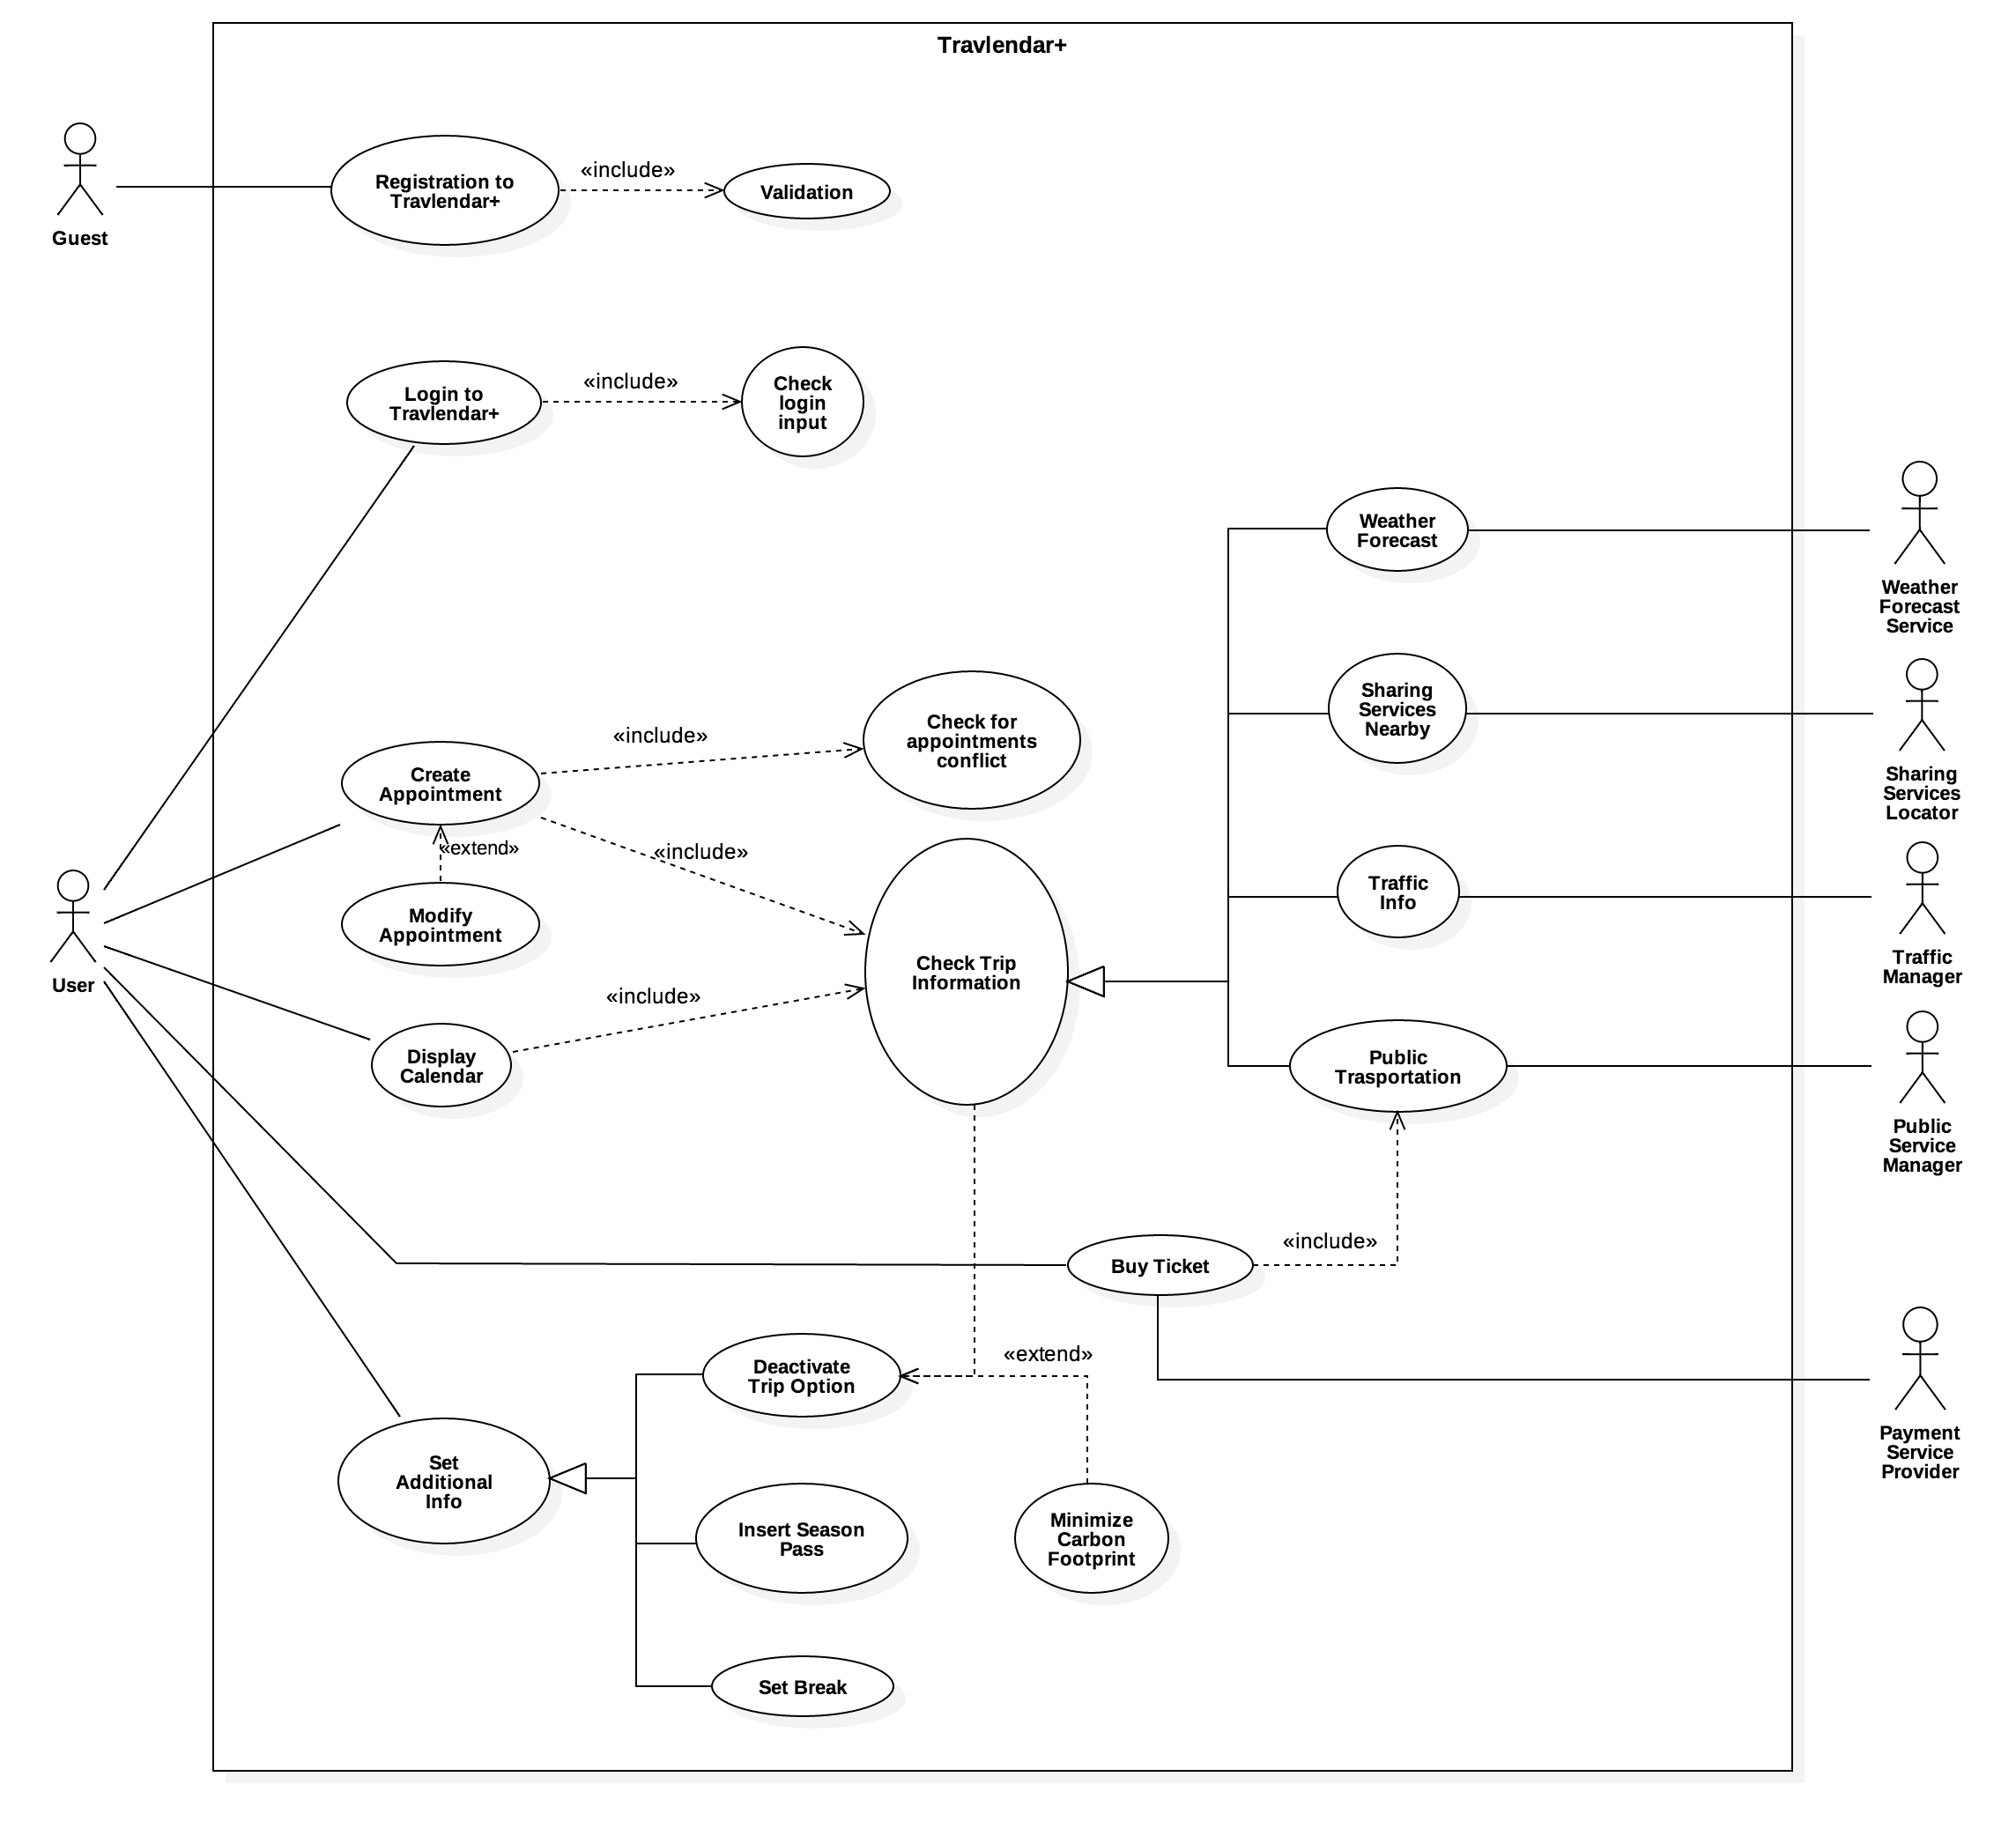
\includegraphics[width=\textwidth]{img/uml/useCase.png}
	
	\vfill
	
%%% CREATE A NEW EVENT %%%	
	\paragraph{Use Case 1: Create a New Event}
	
		\begin{tabular}{| l | p{0.8\textwidth} | }
			\hline
			\hline
			Actor	&		User. \\
			\hline
			Input Condition		&		User is already logged in into \textit{Travlendar+}. \\
			\hline
			Event Flow		&		\begin{enumerate}
												\item User click on "\textit{create event}".
												\item User set day, time, place, and event type.
												\item System checks if the new event overlap with already existing events or lunch period.
												\item	 System calculate, ranks and shows multiple solution depending on user travelling preferences.
												\item User select one solution as preferend one.
											\end{enumerate} \\
			\hline
			Output Condition		&		\textit{Tralvendar+} shows calendar main page with the new event. \\
			\hline		
			Exception		&		\begin{itemize}
											\item[-] Created event overlaps with already existing events.
											\item[-] There are no feasible solution.
										\end{itemize} \\
			\hline
			\hline
		\end{tabular}


%%% MODIFY EVENT %%%

	\paragraph{Use Case 2: Modify Event}
	
		\begin{tabular}{| l | p{0.8\textwidth} | }
			\hline
			\hline
			Actor	&		User. \\
			\hline
			Input Condition		&		\begin{itemize}
													\item[-] User is already logged in into \textit{Travlendar+}.
													\item[-] Event Already Exists.
												\end{itemize} \\
			\hline
			Event Flow		&		\begin{enumerate}
												\item User click on "\textit{Event}".
												\item User starts modifying process.
												\item System checks if the new event overlap with already existing events or lunch period.
												\item	 System calculate, ranks and shows multiple solution depending on user travelling preferences.
												\item User select one solution as preferend one.
											\end{enumerate} \\
			\hline
			Output Condition		&		\textit{Tralvendar+} shows calendar main page, with the updated event. \\
			\hline		
			Exception		&		\begin{itemize}
											\item[-] Created event overlaps with already existing events.
											\item[-] There are no feasible solution.
										\end{itemize} \\
			\hline
			\hline
		\end{tabular}
		
		
%%% INSERT PAYMENT METHOD%%%

	\paragraph{Use Case 3: Insert Payment Method}
	
		\begin{tabular}{| l | p{0.8\textwidth} | }
			\hline
			\hline
			Actor	&		User. \\
			\hline
			Input Condition		&		\begin{itemize}
													\item[-] User is already logged in into \textit{Travlendar+}.
													\item[-] Credit Card isn't already inserted on the system.
												\end{itemize} \\
			\hline
			Event Flow		&		\begin{enumerate}
												\item User click on "\textit{Preferences}" and then on "\textit{Payment Methods}".
												\item User sets all the credit cards info.
												\item System checks and validate provided informations.
											\end{enumerate} \\
			\hline
			Output Condition		&		\textit{Tralvendar+} returns to \textit{Payment Methods} page showing added card as a valid payment method. \\
			\hline		
			Exception		&		Credit card given informations are invalid. \\
			\hline
			\hline
		\end{tabular}

%%% BUY TICKET %%%

	\paragraph{Use Case 4: Buy Public Transportation Ticket}
	
		\begin{tabular}{| l | p{0.8\textwidth} | }
			\hline
			\hline
			Actor	&		User. \\
			\hline
			Input Condition		&		\begin{itemize}
													\item[-] User is already logged in into \textit{Travlendar+}.
													\item[-] A \textit{payment method} is already available.
												\end{itemize} \\
			\hline
			Event Flow		&		\begin{enumerate}
												\item User click on "\textit{Buy Ticket}".
												\item System shows available public trasportation services.
												\item User selects a ticket.
												\item	 System starts perchause transaction.
											\end{enumerate} \\
			\hline
			Output Condition		&		Based on public transportation service, User receives a valid ticket. \\
			\hline		
			Exception		&		Transaction doesn't work. \\
			\hline
			\hline
		\end{tabular}

%%%  RESERVE SHARING SERVICE %%%

	\paragraph{Use Case 5: Reserve a \textit{Sharing Service} resource}
	
		\begin{tabular}{| l | p{0.8\textwidth} | }
			\hline
			\hline
			Actor	&		User. \\
			\hline
			Input Condition		&		\begin{itemize}
													\item[-] User is already logged in into \textit{Travlendar+}.
													\item[-] A \textit{payment method} is already available.
													\item[-] User is in the \textit{influence zone}
												\end{itemize} \\
			\hline
			Event Flow		&		\begin{enumerate}
												\item User click on "\textit{Reserving Service}".
												\item System connects to available \textit{Sharing Service} resources.
												\item System ranks per distance all the freasible recources and shows them on a map centered on User position.
												\item User chooses one on the possible solutions.
												\item	 System reconnects to selected \textit{Sharing Service}, and starts the reserving procedure.
											\end{enumerate} \\
			\hline
			Output Condition		&		User is shown the correct reservation result and the time needed to reach the resource. \\
			\hline		
			Exception		&		Reservation procedure doesn't end well. \\
			\hline
			\hline
		\end{tabular}
		
		
%%%  SET TRIP PREFERENCES%%%

	\paragraph{Use Case 6: Set Trip Preferences}
	
		\begin{tabular}{| l | p{0.8\textwidth} | }
			\hline
			\hline
			Actor	&		User. \\
			\hline
			Input Condition		&		User is already logged in into \textit{Travlendar+}. \\
			\hline
			Event Flow		&		\begin{enumerate}
												\item User click on "\textit{Preferences/Trip}".
												\item System shows all the possible preferences.
												\item User pins prefered options.
											\end{enumerate} \\
			\hline
			Output Condition		&		\begin{itemize}
													\item[-] User returns to Caledar page.
													\item[-] System recalculate all future trip solution according to User preferences.
													\item[-] User is informed of particular problem
												\end{itemize} \\
			\hline
			Exception		&		User unpins all the possible preferences. \\
			
			\hline
			\hline
		\end{tabular}
		
		
%%%  SET LUNCH BREAK %%%

	\paragraph{Use Case 7: Set Lunch Break Period}
	
		\begin{tabular}{| l | p{0.8\textwidth} | }
			\hline
			\hline
			Actor	&		User. \\
			\hline
			Input Condition		&		User is already logged in into \textit{Travlendar+}. \\
			\hline
			Event Flow		&		\begin{enumerate}
												\item User click on "\textit{Preferences/Lunch Time}".
												\item User select an interval and a minimum lenght for his lunch break.
											\end{enumerate} \\
			\hline
			Output Condition		&		System adds those hours as a special meeting every day in the calendar. \\
			\hline
			\hline
		\end{tabular}


	\subsubsection{Sequence Diagrams}
		\paragraph{Create Event}
	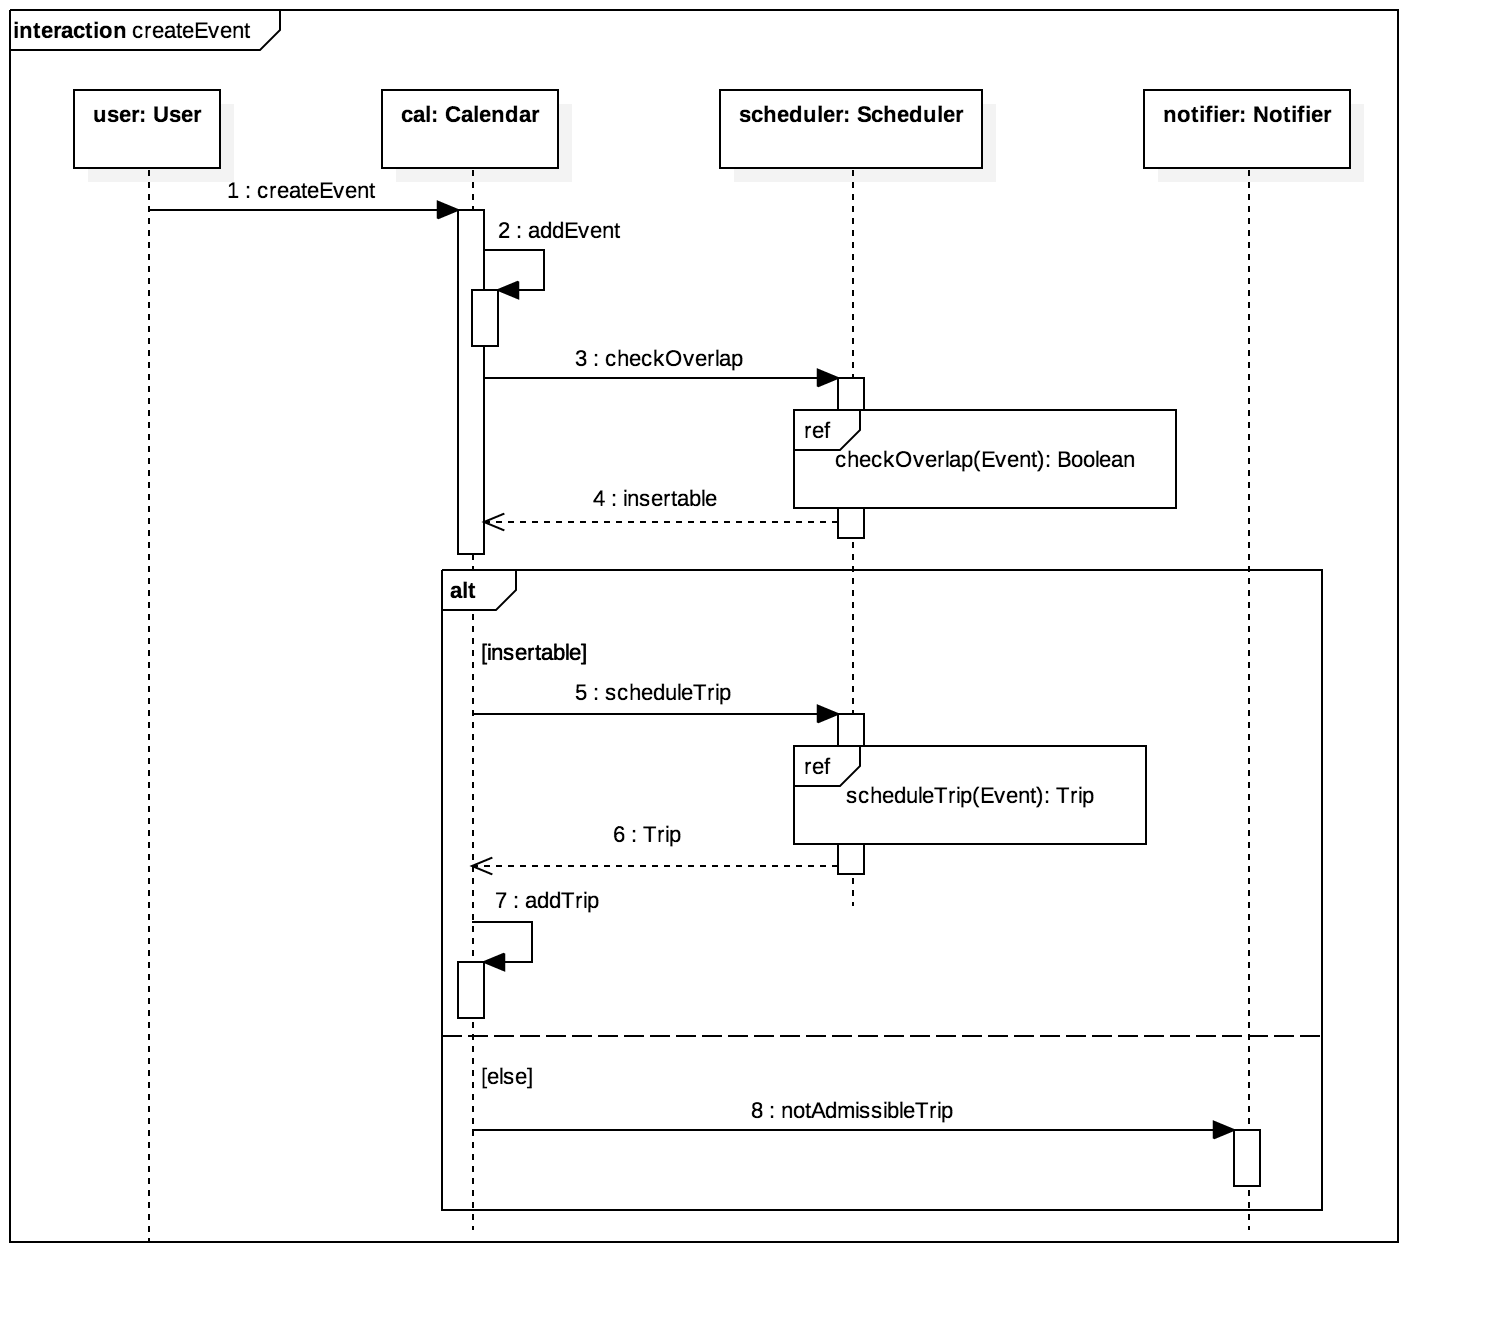
\includegraphics[width=\textwidth]{uml/sequenceDiagrams/createEvent}
	\vfill
	
\paragraph{Subsquence: Check for Overlapping event}
	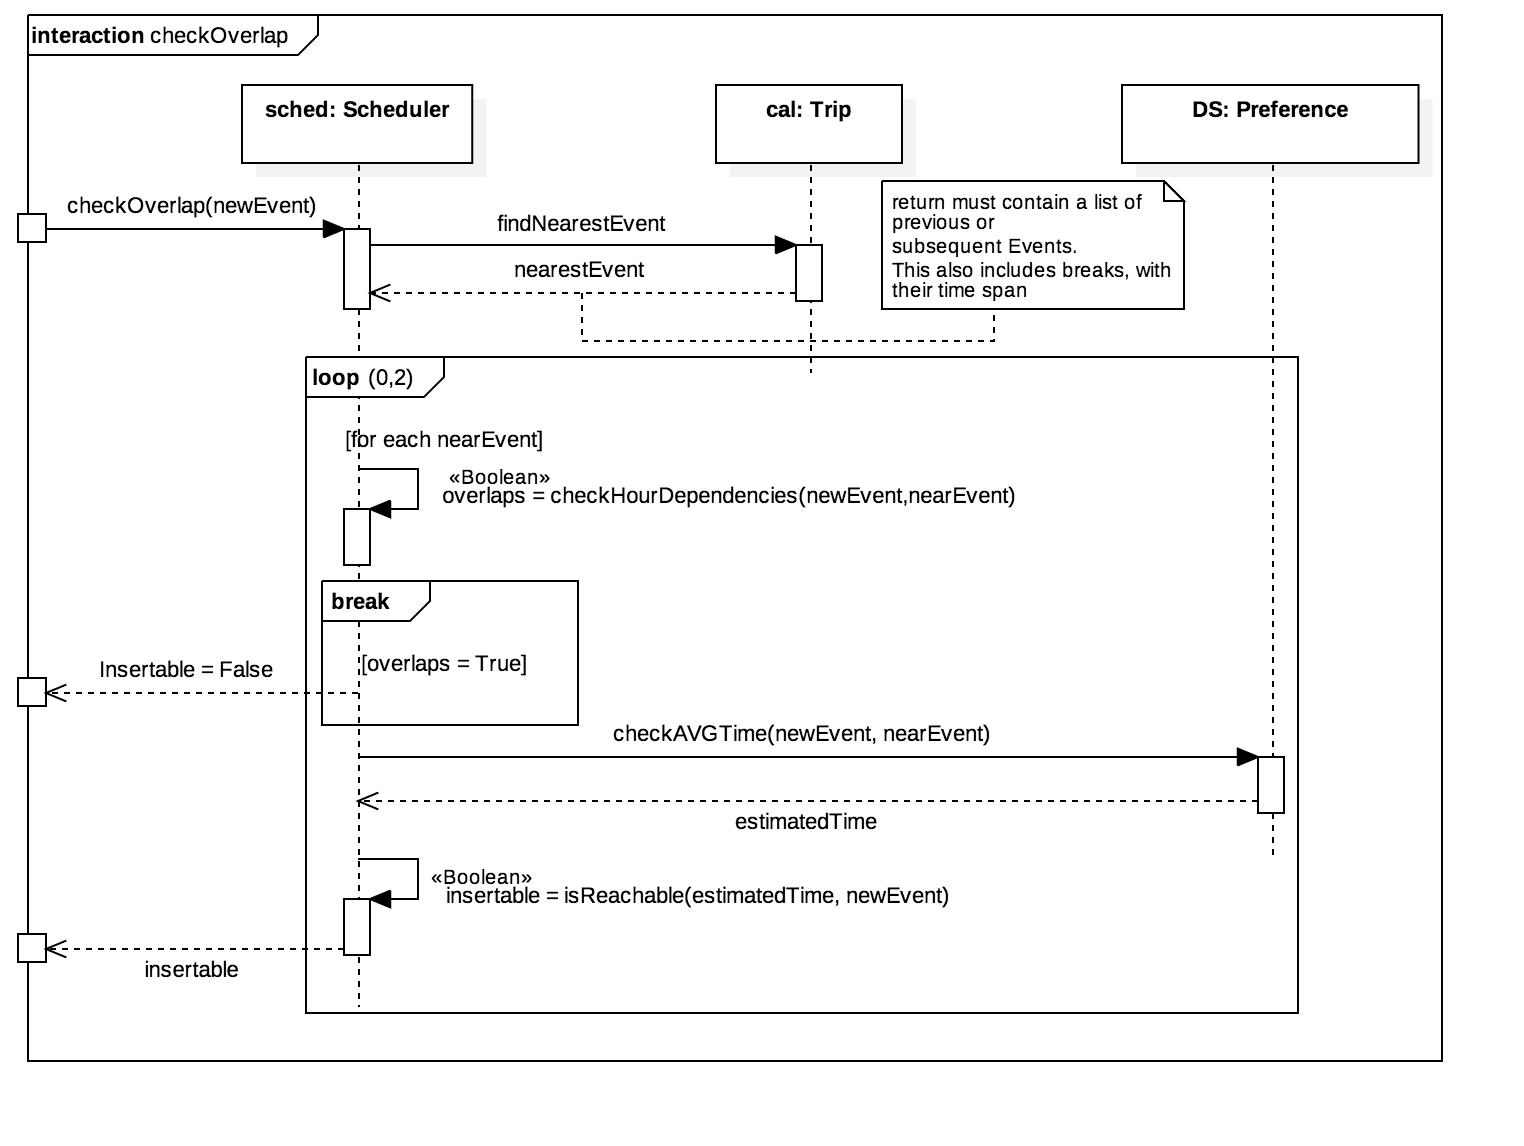
\includegraphics[width=\textwidth]{uml/sequenceDiagrams/checkOverlap}
	\vfill
		
\paragraph{Subsquence: Schedule a Trip}	
	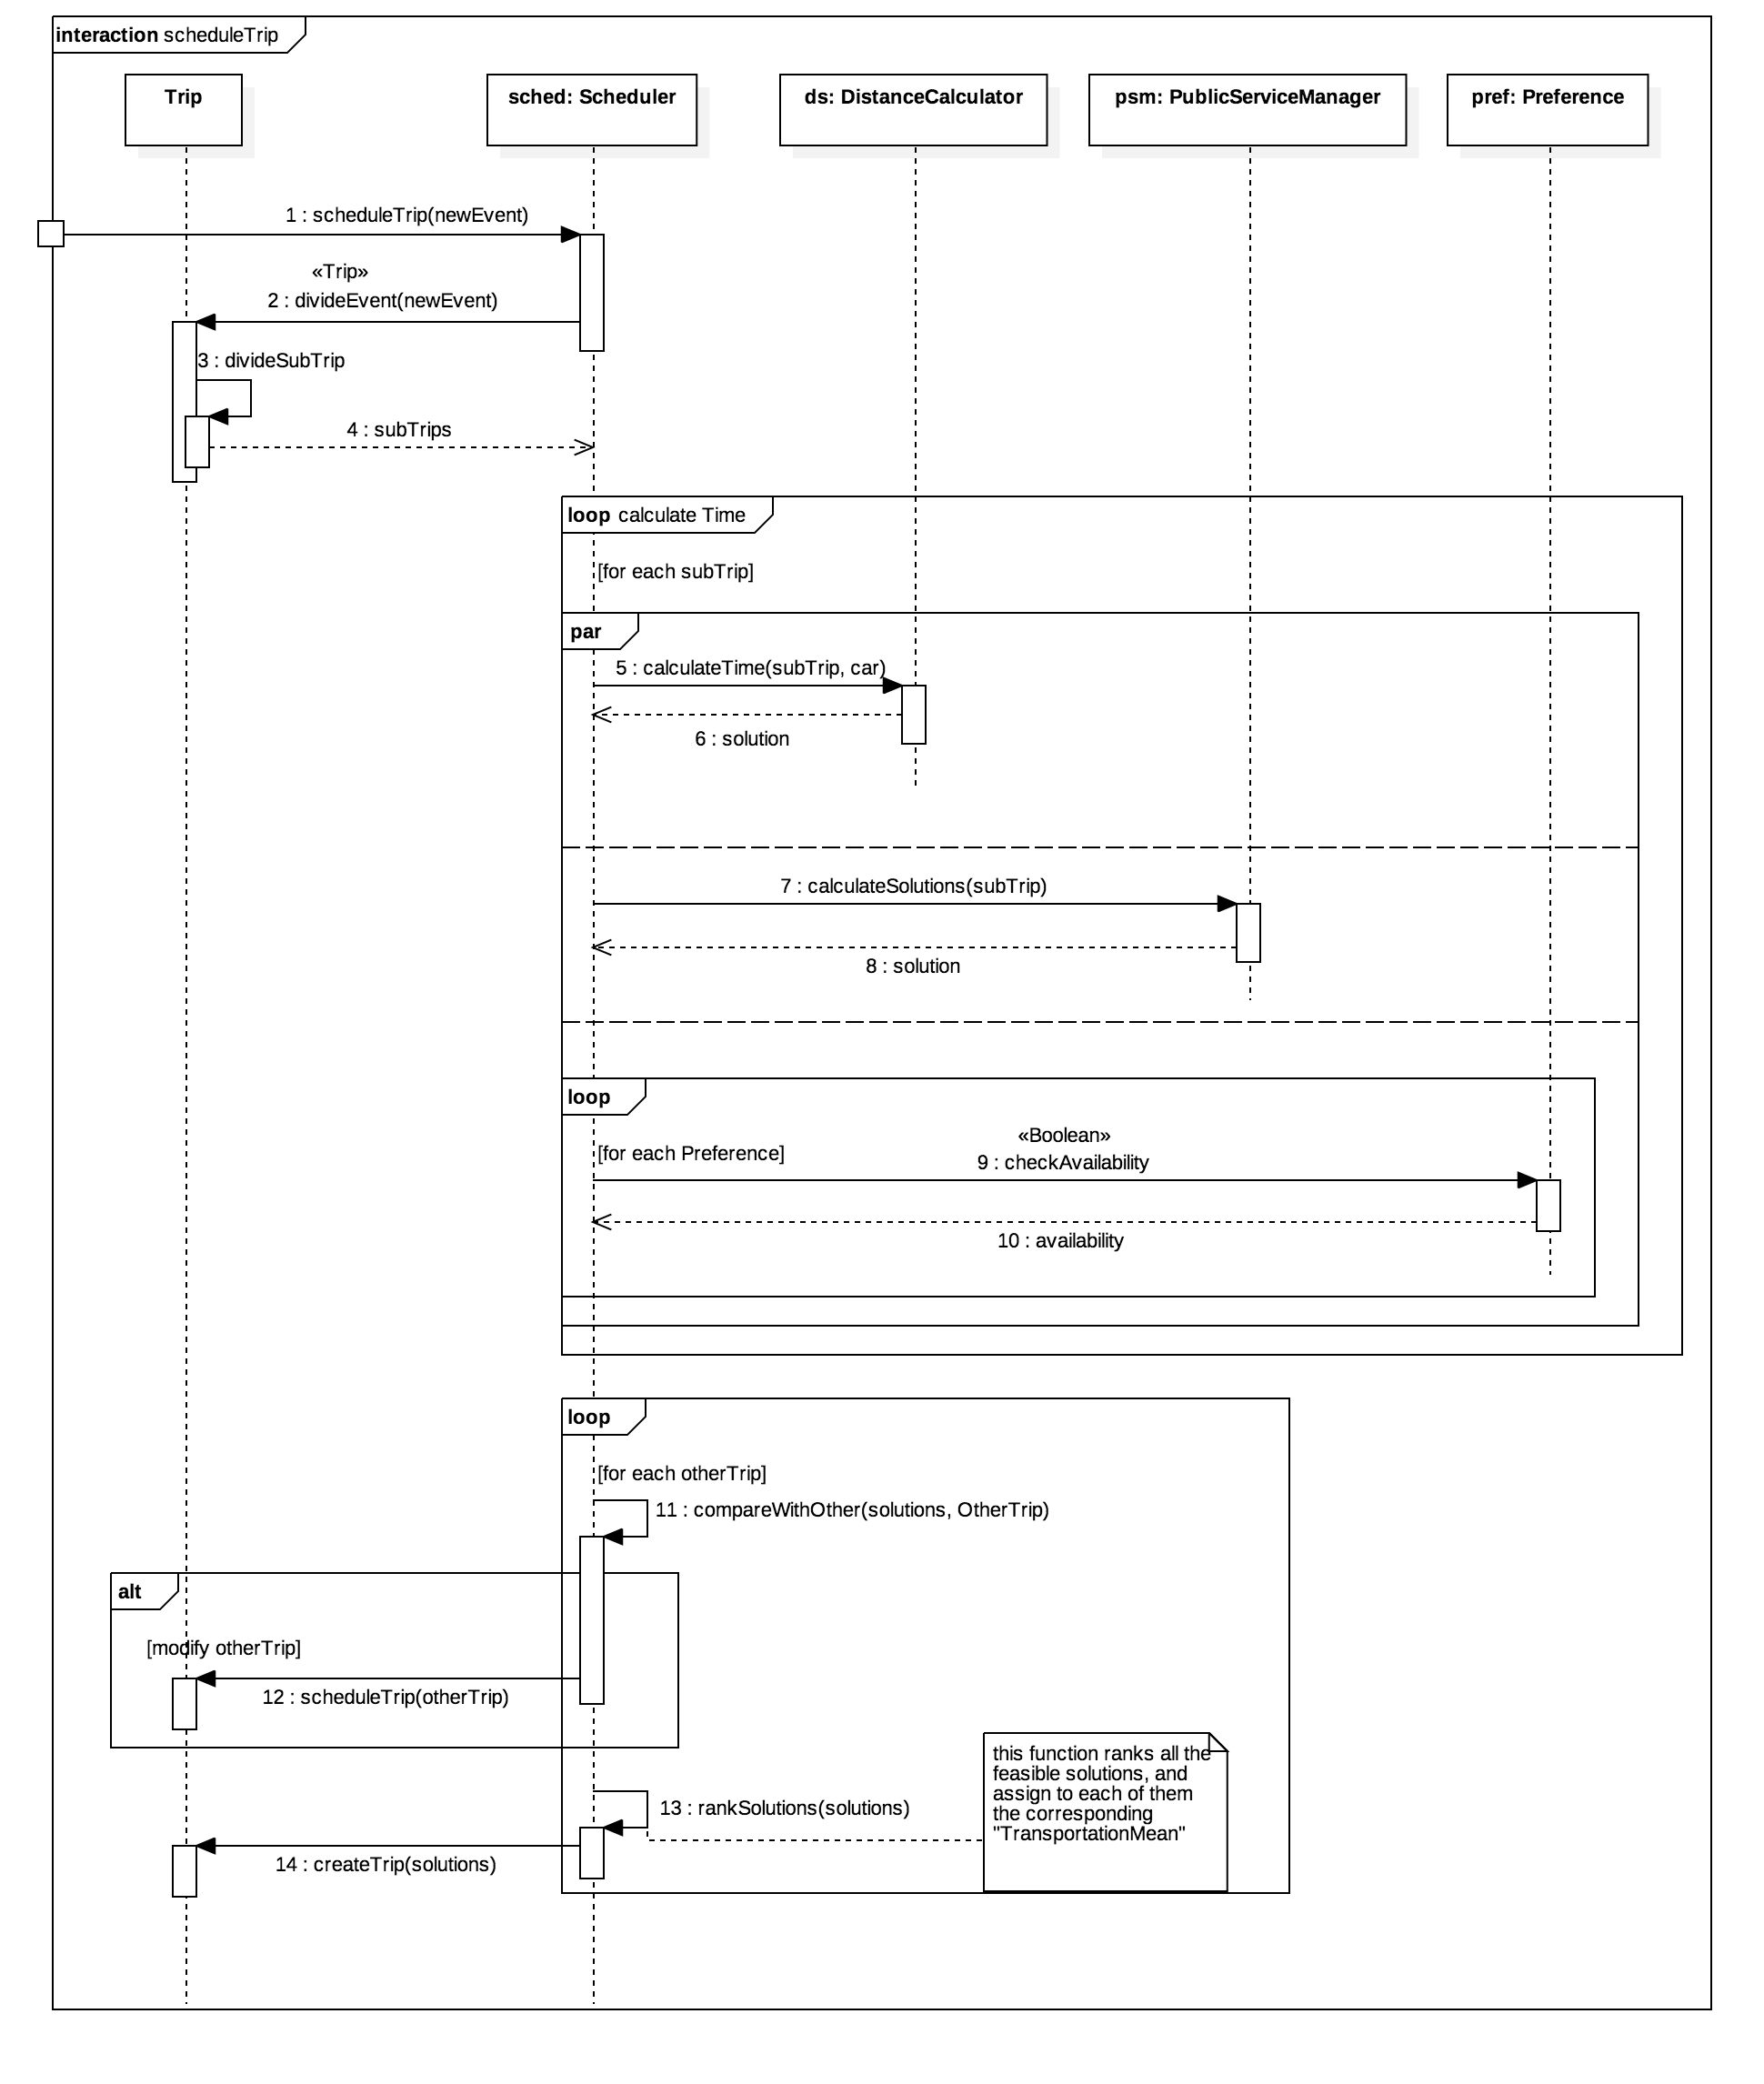
\includegraphics[width=\textwidth]{uml/sequenceDiagrams/scheduleTrip}
	\vfill		
			
%%% C %%%
\subsection{Performance Requirements}

	This section is useful to see how the application manages statical and dynamical non-functional requirements in terms of quantity and quality. 
	In particular:
	\begin{description}
		\item[Static Non-Functional Requirements]	\vfill
		\hfill
		\begin{enumerate}
			\item Application was developed to handle until 50.000 users simultaneously.
			\item Mobile application must run on two most important operative system: iOS and Android.
		\end{enumerate}
		
		\item[Dynamic Non-Functional Requirements] \vfill
		\hfill
		\begin{enumerate}
			\item 98\% of the requests shall be processed in less than 2 second.
			\item The system should be available 99.8\% of the time in one year.
		\end{enumerate}			

	\end{description}
		
		
%%% D %%%	
\subsection{Design Constraints}
		\begin{description}
			\item[Standards compliance]
				The system must require User’s location to work, so the application asks for it according to privacy laws the first time the user runs the application. The payment system is guaranteed by the corresponding external application, so \textit{Travlendar+} doesn’t ask users for their credit card number.

			\item[Hardware limitations]
				Mobile app:
				\begin{itemize}
					\item Space for app package.
					\item 3G connection or better.
					\item GPS.
				\end{itemize}

			\item[Any other constraint]
				No further constraints are imposed.
\end{description}
		
%%% E %%%		
\subsection{Software System Attributes}
	\subsection(Sofware System Attributes)

